
\section{Background and Related Work}
\label{sec:backgr-relat-work}

% REMOVED. IT IS UNNECESSARY (OVERLAPS WITH INTRODUCTION) AND THE
% PAPER IS VERY LONG.
%
% As we mentioned in the introduction, both our group and others have
% made attempts to provide intelligent support in
% ELEs~\cite{MiGen-JRPIT,veermans03,AmersiConati09}.
% However, there will always be situations where the intelligent components cannot 
% help the student or that are intentionally left for the teacher to handle. 
% Examples include very specific conceptual difficulties, 
% engagement nudges to prevent students from getting distracted, 
% and whole-classroom support in, for example, plenary discussions based 
% on students' work. In all these situations, the teacher's role is
% indispensable, especially when dealing with younger children. 
% These types of support are necessary for a productive lesson
% in an exploratory learning setting, yet they can become very
% challenging for the teacher. Depending on
% the classroom configuration, the teacher cannot see all the 
% students' screens at the same time. 
% Even if that is possible, constant demands by the students 
% for the teacher's attention can make it very difficult 
% to monitor what all students are doing at all times. 
% There is therefore a clear need for computer-based support to
% increase the teacher's awareness of the classroom `state' 
% so that she can intervene as appropriate. 
% %In order to design these tools we followed a user-centred approach to
% %derive teacher's requirements in the form of usage scenarios. These
% %are presented in Section~\ref{sec:methodology} whereas the tools are
% %described in more detail in Section~\ref{sec:teach-assist-tools}. 

% In sub-section~\ref{sec:migen-system} we present the MiGen
% system that provides the context in which we have designed and developed 
% a set of Teacher Assistance (TA) tools that aim to assist the
% teacher in focussing her attention across the class and to inform the
% teacher's interventions to support students as they are working in the ELE. 
% We present the MiGen system context in order to help the reader understand 
% our particular case study and to provide a glimpse of the open-ended nature 
% of the activities that students undertake.  In sub-section~\ref{sec:related}
% we present related work.

In sub-section~\ref{sec:migen-system} we present the MiGen
system context in order to help the reader understand 
our particular case study and to provide a glimpse of the open-ended nature 
of the activities that students undertake.  In sub-section~\ref{sec:related}
we present related work.

\subsection{The MiGen system}
\label{sec:migen-system}

The MiGen project (http://www.migen.org) has designed and developed an
intelligent, exploratory environment to support 11 to 14-year-old
students learning of algebraic generalisation.
Using a mathematical microworld called the {\em eXpresser}, students 
are asked to construct two-dimensional tiled models and associated
algebraic rules. In order to build their model, students need to
create `building blocks' out of unit-square coloured tiles depending
on their perception of the model's structure, 
and to repeat each building block in order to form a `pattern'
which forms part of their overall model. 
The algebraic rules they are asked to construct relate 
to the number of tiles of each colour required to paint each 
pattern and their model overall. 
Each building block is made up of a group of
tiles, and can be repeated horizontally, vertically or diagonally to
contribute to the construction of a `pattern'. 
For example, Figure~\ref{fig:example}
shows an example model that students may be asked to construct. 
They may do so by creating building blocks to
generate the centres of the flowers, the petals, and the stalks, 
that they will then repeat to make the yellow, red and green patterns,
respectively. They will be nudged towards deriving rules 
for the number of red tiles and the number of green tiles required 
to paint their model for a given number of yellow tiles.

\begin{figure}[htbp]
  \centering
  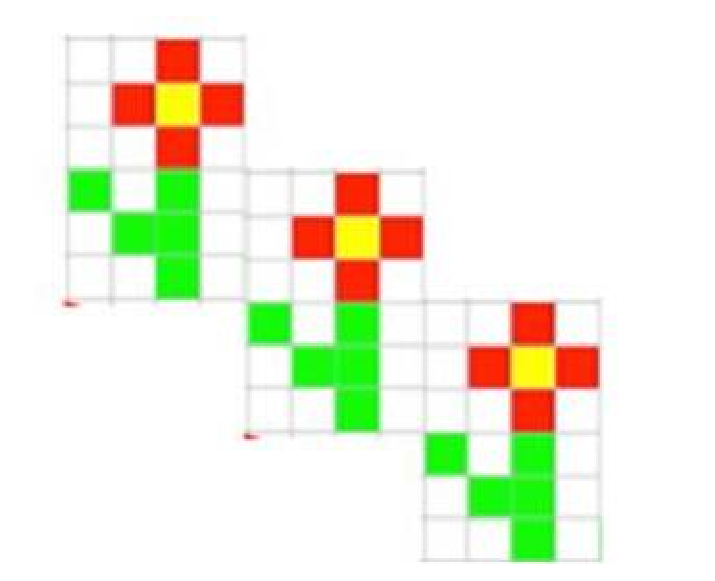
\includegraphics[width=6cm]{gfx/example.eps}
  \caption{An example model that students may be asked to construct in
    eXpresser} 
  \label{fig:example}
\end{figure}

Students are prompted by the eXpresser to check that their models and 
rules are {\em general}, which they can accomplish by making appropriate use of
variables. For example, constructing the model in Figure~\ref{fig:example} requires
one variable --- for the number of yellow tiles. If the model has been
constructed generally by the student, changing the value of this variable
will lead to the whole model being updated correctly and also
still being correctly and fully coloured. The eXpresser has an
`animation' facility which allows students to explore the generality
of their models and rules. This facility automatically applies
different random values to the variables used by the student and
displays the resulting instances of the model in a separate pane of
their screen.  

Tasks are designed to contextualise students' interaction with the
eXpresser and include a set of goals that students need to achieve,
e.g. `construct your model', `make sure it is correctly coloured',
`check that it animates without messing up', and `check that your
animated model is always correctly coloured'. The task goals are
presented to the student within an {\em Activity Document}, in which
students can tick off goals they believe they have completed, answer
questions relating to the task, and reflect on their construction approach.
We refer the reader to~\cite{Manolis2012Sowing} for further 
details of the eXpresser, its `epistemic affordances' and how it can 
enhance students' understanding of algebraic generalisation 
and to~\cite{MiGen-CAE} for further details of the MiGen system architecture, 
the Activity and Task design tools, and Activity Documents.  

Exploratory Learning Environments such as MiGen's eXpresser
have the potential to support students' exploration while at the same
time fostering progressive building of knowledge. However, the
exploratory nature of the tasks undertaken with eXpresser requires
that personalised feedback is provided to students as they construct
their solutions, and not just at the end of the task. This feedback
includes prompts to help students engage with a task, 
guide them towards successful completion of the task, 
and generalise their solutions~\cite{MiGen-CAE,MiGen-JRPIT}. 
This feedback is generated by another
component of the MiGen system, the {\em eGeneraliser}, based on an
analysis of students' actions in the eXpresser. 
% and in MiGen we provide personalised feedback to students as they are
% undertaking their constructions, in the form of a series of prompts
% and nudges that help students reflect upon their interactions and
% guide them towards successful completion of the task. 
%
The aim of the feedback is to balance students' freedom to explore 
while at the same time providing sufficient support to ensure that 
learning is being achieved. We refer the reader to~\cite{MiGen-JRPIT} for
details of the design of the eGeneraliser and of the feedback that it
provides to students. 

%\subsection{Our approach - merge with previous}
%\label{sec:our-approach}
 
%In the MiGen system, 

As students are undertaking the task set in the eXpresser, a series
of {\em indicators} are automatically detected by the eXpresser or
inferred by the eGeneraliser and submitted by them to the MiGen
Server for storage in the MiGen database\footnote{The MiGen software
  comprises the eXpresser running on each student's computer, the TA
  tools running on the teacher's computer, and the MiGen Server and
  database running on a third computer. The MiGen database stores all
  the information produced and required by the eXpresser and the TA
  tools (see ~\cite{MiGen-CAE,IEEE-TLT-TA} for details).}.   
The set of indicators that are meaningful and useful for teachers in
their role in the classroom has been identified through an iterative
process, undertaken collaboratively with our group of teacher
collaborators on the MiGen project (see Section~\ref{sec:methodology}).  

There are two categories of indicators: Task Independent (TI)
indicators refer to aspects of the student's interaction that are
related to the microworld itself and do not depend on the specific task
the student is working on. TI indicators generally refer to a single
action undertaken by the student, such as `placed a tile on the
canvas', `created a building block', `created a pattern'. In contrast,
the detection of Task Dependent (TD) indicators requires 
knowledge of the task the student is working on, may relate
to combinations of student actions, and requires intelligent
reasoning by the system. This reasoning is undertaken by the
eGeneraliser, using a mixture of case-based and rule-based
techniques. Examples of TD indicators are `student has made a
plausible building block for this task', `student has coloured their
pattern generally' and `student has achieved a task goal'. Detailed
discussions of the MiGen's TI and TD indicators and how the latter are
inferred by the eGeneraliser may be found in~\cite{IEEE-TLT-TA}.
 
The TA Tools, described in more detail in Section~\ref{sec:teach-assist-tools},
receive real-time information from the MiGen server relating to
occurrences of TI and TD indicators for each student, and each TA tool
presents a selection of this information in a visual fashion to the
teacher. 
% % REMOVED FOR THE SAKE OF SPACE. SEE ALSO DISCUSSION BELOW (AP NOTE,
% % SG REPLY). 
% % 
% The TA tools include the Student Tracking (ST) tool, the
% Classroom Dynamics (CD) tool and the Goal Achievements (GA) tool. 
% %
% % AP NOTE - N.B. we need enough detail here for the reader to be able to
% % understand Tables 1 and 2, that come before the detailed description
% % of the tools in Section 4! I have added therefore a bit more info
% % here. 
% %
% % SG REPLY - I disagree. I think this is not necessary, so I remove it
% % for the sake of space. Table 1 and 2 are near Section 4, and they
% % actually appear on paper after Section 4 has started. 
% % On a related note, I am not sure Tables 1 and 2 should make
% % reference to the use of the tools... it may be a bit distracting,
% % and overlaps with Section 4.5. 
% %
% The ST tool provides real-time visualisation of the  occurrence of all 
% TI and TD indicators as each student is interacting with eXpresser. 
% Indicators are  coloured Green, Red or Yellow depending on the system's perception
% of whether their occurrence indicates productive interaction,
% unproductive interaction, or interaction that may be productive or
% unproductive depending on context.
% %
% % , showing these in one column of the display for each
% % student, with time increasing downwards, and new information being
% % added at the bottom of the display (see Figure\ref{eee}). Indicators
% % are coloured Green if the occurrence of such an indicator indicates
% % that the actions of the student are consistent with what would be
% % expected by the system from constructive interaction, Red if the
% % occurrence of such an indicator is regarded by the system as an
% % obstruction to constructive interaction, Yellow if the occurrence of
% % such an indicator indicates an aspect of the student's interaction
% % that may be positive or negative depending on the context, and Blue
% % for indicators that represent feedback generated by the system for the
% % student. Further details relating to Figure 2 and the ST tool are
% % given in Section~\ref{sec:4.1}.
% %
% The CD tool represents each student in the classroom 
% visually as a circle whose colour
% is updated to reflect the current status of the student: 
% active (Green), inactive (Amber), or waiting for help from the teacher (Red). 
% %
% % A small subset of the total TI/TD indicators are required to update this
% % information, namely the indicators relating to students'
% % activity/inactivity and students' usage of the eXpresser's help
% % facility. If the teacher clicks on one of the circles in the CD
% % display, that student's current model and rule, as currently being
% % worked on by the student in the eXpresser, is displayed to the teacher
% % (see Figure\ref{fff}).
% % 
% % The teacher can also select to see a summary of the goal achievement
% % information within the CD tool by switching on a feature that displays
% % within the student's circle the number of goals achieved so far as a
% % fraction of the total number of goals e.g. if the student has achieved
% % 2 of a total of 4 task goals, this would show as 2/4� within the
% % student's circle. That feature has been enabled in the display shown
% % in Figure\ref{4r4r}. 
% %
% An optional feature in this tool shows within each student's circle the number of
% goals achieved so far, as a fraction of the total number of goals of the task. 
% %
% The Goal Achievements (GA) tool shows in more detail the progress of each
% student on achieving each of the goals of the task. 
% % 
% % It tracks just one of the indicators - `student has achieved
% % a task goal' - and shows visually, in the form of one row per student,
% % the achievement of each task goal by each student (see Figure
% % 5). Tasks shown as Green are currently achieved, those shown as White
% % are currently not achieved, and those shown as Amber were achieved at
% % some point during the student's construction but are not being
% % achieved by the current model.


%%% End:
\subsection{Related Work}
\label{sec:related}

To our knowledge, MiGen's TA tools (preliminary results were published
in~\cite{TA-ECTEL}) represent the first work that is targeted at
notifying teachers of students’ progress and state during constructionist
learning activities in the classroom, notifying the teacher of
students’ attainment of key indicators, and aiming to inform the
teacher’s own interventions in the class. This novelty of our TA tools
has presented a number of methodological challenges, which we discuss
in Section 3. In the last two years, several similar initiatives have
appeared, including the work at the Metafora
project~\cite{Dragon13}\ednote{SG: I think there was a better paper,
  but I cannot find it now. Maybe MM can help.}, although their
feedback focuses on the statistics of the interaction (e.g.~how often
did the student produce a certain kind of indicator, 
c.f.~\cite{Gueraud09}). As explained in
this paper, we believe that immediate on-line feedback is
more valuable to teachers for orchestrating the use of technologies in
the classroom, an approach recently shared by~\cite{Gutierrez12}
(inspired by early work by~\cite{Yardi08}). Gutierrez focuses on
progress measurement and whether students are stuck in the context of
programming labs. 

The trend towards teacher support appears to grow
also in the learning analytics community
(see for example~\cite{Crespo12,Zaldivar12,Pardo12}, and there is high
synergetic potential between their work and the work reported here.
Other related initiatives include 
using Web log data generated by course management systems
(e.g.~WebCT) to help instructors become aware of students’
activities in distance learning classes~\cite{Mazza07}; post-analysis of
the system's data logs for helping teachers understand students'
behaviour in adaptive tutorials~\cite{BenAnim08}; or providing
awareness information to teachers so as to support their role as 
moderators of multiple e-discussions~\cite{Wichmann09}; although none of them
focuses on exploratory learning activities or environments. 
Particulartly interesting is the work described in 
is~\cite{Avouris08}, that uses tools to analyse CSCL 
synchronous interaction to help the teacher; their use of ``rules'' to
find specific landmarks in the interaction bears some
similarity to the search of indicators we report here. 


% Stefan Weinbrenner, Jan Engler, Astrid Wichmann, Ulrich Hoppe
% Monitoring and Analyzing Students' Systematic Behaviour by Agents -
% The SCY Pedagogical Agent Framework. Proceedings of the 5th European
% Conference on Technology Enhanced Learning (EC-TEL 2010), Barcelona,
% ES, 2010

% -- this I think is one of those mentioned at the top
% Stefan Weinbrenner, Jan Engler, Astrid Wichmann, Ulrich Hoppe
% Monitoring and Analyzing Students' Systematic Behaviour by Agents -
% The SCY Pedagogical Agent Framework. Proceedings of the 5th European
% Conference on Technology Enhanced Learning (EC-TEL 2010), Barcelona,
% ES, 2010


% Discussion here also of other related work on: 
% \begin{itemize}
% \item  interaction analysis
% \item  work on CSCL (even if we are not targetting collaboration here)
%   to support teachers 
% \item  work on teachers’ tools for moderating online discussions and
%   argumentation 
% \item  other tools for learning
% \item Argonaut's teacher tools (Astrid Wichman, Ulrich Hoppe)
% \end{itemize}


%%% Local Variables:
%%% mode: latex
%%% TeX-master: "main"